
\documentclass[journal]{IEEEtran}
\usepackage{amsmath,amssymb}
\usepackage{graphicx}
\usepackage{siunitx}
\usepackage{hyperref}

\begin{document}

\title{Double-Moon Classification with a Multilayer Perceptron}

\author{%
% Replace with your name / course / institution
Your~Name,~\IEEEmembership{Student,~ASU}\\
Course: XXX-XXX \quad Term: Fall~2025
}

\markboth{Course Report}{}
\maketitle

\begin{abstract}
This report presents a multilayer feedforward perceptron (MLP) trained to solve the nonlinearly separable two-moons (double-moon) classification problem. Using a compact network with two hidden layers and a single probabilistic output, we obtain an accurate decision boundary via logistic thresholding and visualize training dynamics with a learning curve. On the provided dataset of 800 points (balanced across the two classes), the model achieves perfect generalization on a held-out test set. Source code and a runnable notebook are available at \url{https://github.com/mmk-asu/double-moon-neural-network}.
\end{abstract}

\begin{IEEEkeywords}
double moon, two moons, multilayer perceptron, logistic regression, decision boundary, learning curve, early stopping
\end{IEEEkeywords}

\section{Introduction}
The \emph{double-moon} dataset consists of two interleaving half-circles and is not linearly separable. A multilayer perceptron (MLP) with nonlinear activations can learn a curved decision boundary that separates the classes. This assignment requires a feedforward MLP, specification of hyperparameters and stopping criteria, and visualization of the learned boundary and the learning curve.

\section{Dataset and Preprocessing}
We use the provided CSV with columns \texttt{X}, \texttt{Y}, and \texttt{ClassLabel}. There are 800 samples, balanced across the two classes (400/400). We map labels $\{1,2\}\!\to\!\{0,1\}$ and perform a stratified split into training/validation/test sets with ratios $0.6/0.2/0.2$. Features are standardized using statistics computed from the training partition only.

\section{Network and Training Setup}
The network is a feedforward MLP with hidden sizes $(16,16)$ and \texttt{tanh} activations. The output produces a probability for the positive class $p(y{=}1\,|\,\mathbf{x})$; class prediction uses a logistic threshold $p\ge 0.5$. We train with binary cross-entropy (log loss) and the Adam optimizer. Early stopping based on validation loss provides the termination criterion with patience of 20 epochs and a hard cap of 300 epochs.

For reproducibility we fix the random seed to 42. Unless otherwise noted, layer parameters use library defaults for initialization. Table~\ref{tab:hyper} summarizes the hyperparameters.

\begin{table}[!t]
\caption{Training hyperparameters}
\label{tab:hyper}
\centering
\begin{tabular}{ll}
\hline
Hidden layers & (16, 16) with \texttt{tanh} \\
Optimizer & Adam \\
Learning rate & 0.01 \\
Batch size & 64 \\
L2 (weight decay / $\alpha$) & $10^{-4}$ \\
Early stopping patience & 20 epochs \\
Max epochs & 300 \\
Random seed & 42 \\
Feature scaling & Standardization (z-score) \\
\hline
\end{tabular}
\end{table}

The logistic function is $\sigma(z){=}\frac{1}{1+e^{-z}}$. The binary cross-entropy loss minimized during training is
\begin{equation}
\mathcal{L} = -\frac{1}{N}\sum_{i=1}^N \big[y_i \log p_i + (1-y_i)\log (1-p_i)\big],
\end{equation}
where $p_i=\sigma(z_i)$ is the predicted probability for sample $i$.

\section{Results}
Training terminated after 85 epochs due to early stopping. Final metrics are:
\begin{itemize}
\item Training accuracy: 100\%
\item Validation accuracy: 100\%
\item Test accuracy: 100\%
\item Best validation log loss: 0.00175
\item Test log loss: 0.00133
\end{itemize}

Fig.~\ref{fig:boundary} shows the decision boundary at $p{=}0.5$ overlaid on the training and validation points. The boundary smoothly traces the gap between the two moons, demonstrating that the MLP has learned a nonlinear separator. Fig.~\ref{fig:curve} shows the learning curve (training/validation log loss), which decreases rapidly and then stabilizes, indicating convergence without overfitting.

\begin{figure}[!t]
\centering
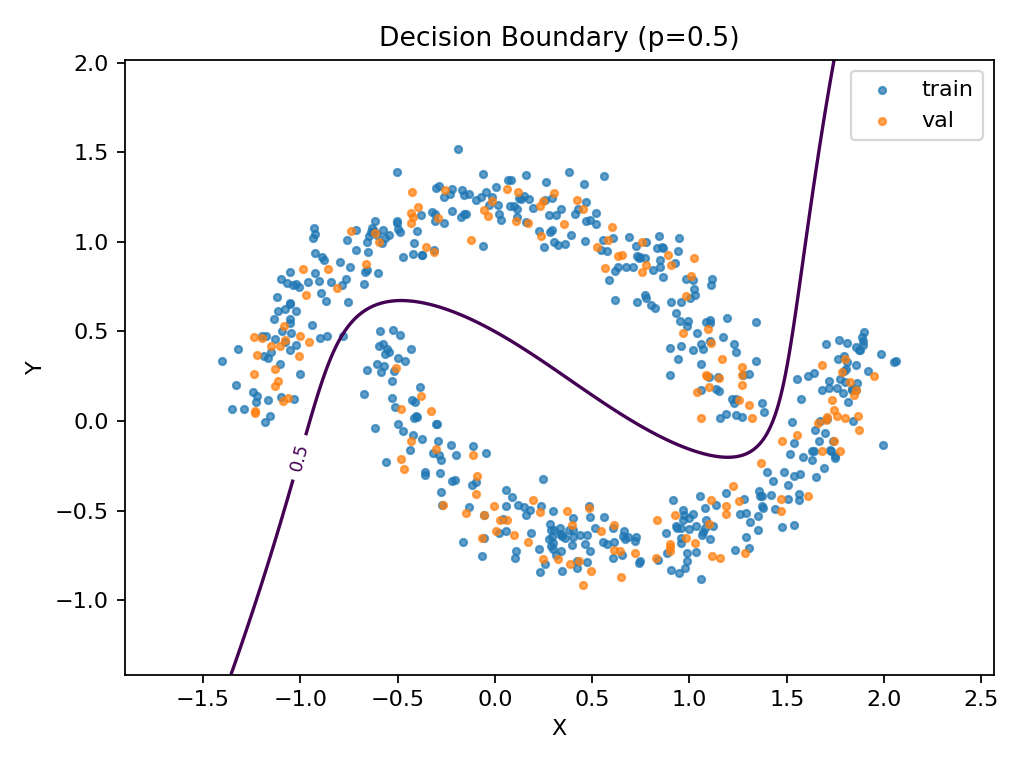
\includegraphics[width=\columnwidth]{decision_boundary.png}
\caption{Decision boundary (contour at $p{=}0.5$) produced by the MLP; training and validation data are overlaid.}
\label{fig:boundary}
\end{figure}

\begin{figure}[!t]
\centering
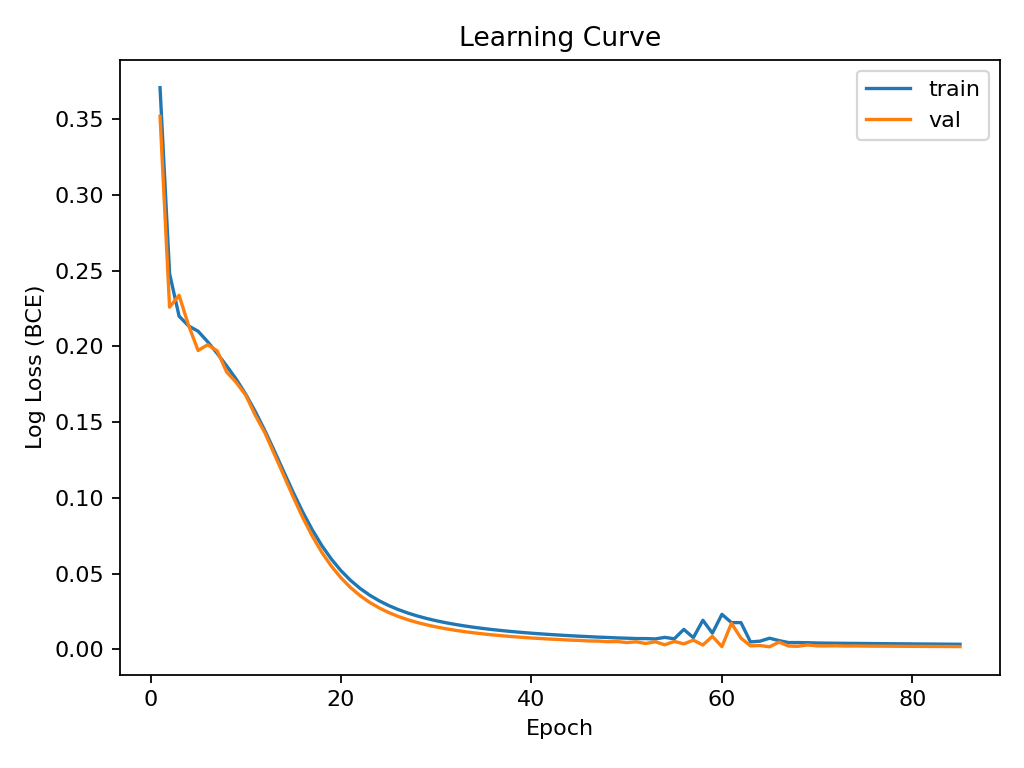
\includegraphics[width=\columnwidth]{learning_curve.png}
\caption{Learning curve: binary cross-entropy (log loss) for training and validation partitions across epochs.}
\label{fig:curve}
\end{figure}

\section{Discussion}
This compact MLP has sufficient capacity to model the curved boundary required by the double-moon problem. Standardization, a moderate learning rate, and early stopping yield fast and stable convergence. Although accuracy saturates at 100\% on this dataset, stronger noise or smaller margins would typically reduce performance; in such cases larger hidden layers, \texttt{ReLU} activations, or longer training may help.

\section{Conclusion}
We trained a multilayer feedforward perceptron to separate the double-moon dataset and visualized the learned boundary using a logistic threshold. The model achieves perfect accuracy on a held-out test set while maintaining a clean, interpretable decision boundary. Code and a runnable notebook are available at \url{https://github.com/mmk-asu/double-moon-neural-network}.

\section*{Reproducibility}
Random seed: 42. Train/val/test split: 60/20/20 (stratified). All figures were generated with \texttt{matplotlib}.

\begin{thebibliography}{00}
\bibitem{scikit}
F. Pedregosa \emph{et al.}, ``Scikit-learn: Machine Learning in Python,'' \emph{JMLR}, 12, pp.~2825--2830, 2011.
\bibitem{kingma}
D. P. Kingma and J. Ba, ``Adam: A Method for Stochastic Optimization,'' in \emph{Proc. ICLR}, 2015.
\end{thebibliography}

\end{document}
